\documentclass[a4paper,titlepage,12pt]{article}
\usepackage[italian]{babel}
\usepackage{appendix}
\usepackage{amsmath}
\usepackage{graphicx}
\usepackage{float}
\usepackage{pifont}
\usepackage{hyperref}

\title{Marcello Apocalypse}
\author{Luca Babboni, Federico Bartolini, Samuele De Tuglie, Sara Romeo}

\begin{document}
\maketitle
\tableofcontents

\newpage
\section{Analisi}
L'applicativo proposto consiste nella realizzazione di un videogioco turn-based, dove il protagonista (Marcello) si ritrova a fuggire da un apocalisse zombie. Questo corre in un tombino ed entra in una fognatura: il giocatore dovrà superare le varie stanze uccidendo gli zombie nemici, raccogliendo artefatti e armi. Il gioco termina nel momento in cui si vince trovando l'uscita o si perde nel momento in cui esaurisce la vita disponibile.

\subsection{Requisiti}
\subsubsection*{Requisiti funzionali}
\begin{itemize}
    \item Gestione del turno
    \item Differenti tipi di armi
    \item Differenti tipi di nemici
    \item Sistema di cura 
    \item Creazione e collegamento di stanze 
    \item GUI minimale 
    \item Gestione di oggetti (modificatori di statistiche) 
    \item Struttura del menù di azioni 
\end{itemize}

\subsubsection*{Requisiti opzionali}
\begin{itemize}
    \item Generazione ostacoli al movimento nella mappa 
    \item Gestione dell'inventario (diversi artefatti equipaggiabili)
    \item Effetti sonori
\end{itemize}

\subsection{Analisi e modello del dominio}
Le entità che entrano in gioco all'interno del dominio sono principalmente Marcello, gli zombie nemici, le armi, gli artefatti e le stanze in cui tutte le azioni prendono luogo.
Marcello dovrà essere in grado di passare attraverso un insieme di stanze differenti. In ogni stanza troverà dei nemici da affrontare/evitare che si muoveranno e proveranno ad attaccarlo per eliminarlo. Nelle stanze dovranno esserci artefatti raccoglibili modificatori di statistiche quali la vita, il modo in cui Marcello può spostarsi o il numero di azioni che può compiere in un turno. Per terra si possono trovare anche armi che arrecano danni diversi: una volta giunti sulla casella in cui una di queste si trova, essa sarà scambiata con l'arma correntemente in possesso. Ogni arma permetterà di attaccare in celle diverse. Queste sono rappresentate da artefatti di cambio arma.
\begin{figure}[H]
    \centering
    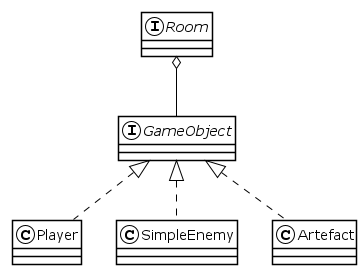
\includegraphics[scale=0.8]{img/uml/Entity.png}
    \caption{Schema UML delle entità del dominio.}
    \label{img:model}
\end{figure}
\noindent I requisiti non funzionali riguardanti
\begin{itemize}
    \item[--] Gestione dell'inventario (diversi artefatti equipaggiabili)
    \item[--] Effetti sonori
\end{itemize}
avrebbero richiesto più tempo rispetto al monte ore previsto: tali feature saranno oggetto di futuri lavori.

\newpage
\section{Design}
\subsection{Architettura}
La scelta per il pattern architetturale è \textit{MVC (model-view-controller)}, in quanto ci ha permesso di separare efficientemente la logica di gioco dalle feature grafiche, gestendo i rapporti tra loro all'interno del controller. 
Nel nostro caso abbiamo creato un'interfaccia per ogni ambito in modo da semplificare le relazioni tra di esse.

\begin{figure}[H]
    \centering
    \includegraphics[scale=0.8]{img/uml/MVC.png}
    \caption{Schema UML del modello MVC.}
    \label{img:model}
\end{figure}

\par \noindent Il punto di ingresso del programma è rappresentato dal game loop, che funge da inizializzatore del gioco e da mediatore tra il view controller e il game controller.
\par \noindent Essendo un gioco turn based gli input arriveranno da parte dei bottoni posti nel Total Panel. È stata ideata l’interfaccia Game controller che si occupa di intercettare gli eventi provenienti dalla view (per esempio la pressione di un bottone), per poi chiamare i rispettivi metodi sul game loop che decideranno come gestirli. Per la maggior parte del gameplay il personaggio dovrà muoversi e attaccare, questo sarà possibile tramite i pulsanti precedentemente citati. In questo caso il game loop passerà la richiesta di azione all’interfaccia game controller che si occuperà invece di incapsulare al suo interno la logica e lo stato della partita, andando ad utilizzare i metodi esposti dal Model. Inoltre quando avviene un cambiamento nello stato della partita che implica un aggiornamento nella parte di View si occuperà di comunicare con quest’ultima notificando il cambiamento.
\par \noindent Total Panel al suo interno incapsula quella che è la parte di view del progetto. Per garantire una facile sostituzione, quest’ultima si interfaccia con view controller, evitando quindi che un cambiamento del blocco view incida sulla parte di controller.
\par \noindent Per una ipotetica sostituzione basterà quindi ricreare la parte di view con una nuova libreria, per poi collegare il gestore delle azioni dei nuovi pulsanti ai rispettivi metodi esposti dal view controller.
\par \noindent Poiché MAP è un gioco turn based quest'architettura permette una facile comunicazione tra i vari elementi  che lo compongono. 
\newpage
\subsection{Design dettagliato}

\subsubsection*{\large \slshape Luca Babboni}
\paragraph{GameObject ed Entity}
\par \noindent \\
\begin{figure}[H]
    \centering
    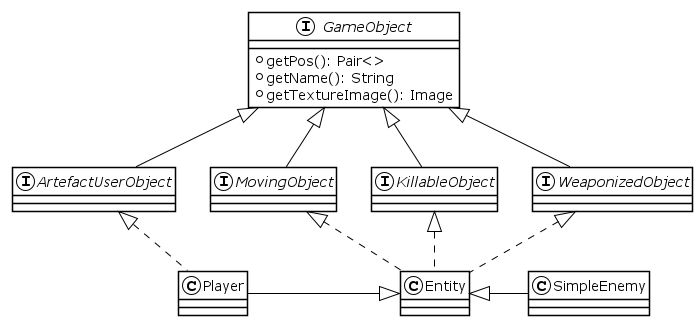
\includegraphics[scale=0.55]{img/uml/GameObject.png}
    \caption{Game Object}
    \label{fig: Game Object}
\end{figure}
\par \noindent Il primo passo per la realizzazione della logica del gioco è stato quello di definire tutti i metodi comuni agli oggetti che saranno poi presenti all’interno dell’area di gioco (player, enemy ed artefatti). Il comportamento è molto diverso per ognuno di loro, ma presentano comunque metodi in comune. Questo ha portato alla creazione dell’interfaccia GameObject. 
\par \noindent L’idea alla base di questa interfaccia è quella di formulare i metodi comuni a tutti gli oggetti rappresentabili, fornendo uno scheletro attorno al quale è possibile costruire oggetti più complessi. 
\par \noindent Il principale vantaggio di questa interfaccia è rappresentato dalla facilità di ampliabilità del progetto. Se ben utilizzata infatti permette la creazione di metodi molto generici nella parte di controller, che possono continuare a funzionare senza modifiche anche in caso di aggiunta di un nuovo componente di gioco. 
\par \noindent Sempre tenendo a mente l’ampliabilità del progetto sono state create diverse interfacce con uno scopo simile a quello dell’interfaccia game object. 
\par \noindent Il personaggio principale condivide alcune funzionalità con i nemici, come ad esempio poter attaccare e muoversi, ma solo il primo può curarsi, usare degli artefatti e muoversi piú volte per turno.
\par \noindent Con quest’ottica ho deciso di suddividere in maniera capillare le interfacce che compongono le entità di gioco.  Questo permette di poter creare entità implementando interfacce fisse, senza per questo limitare le funzionalità di una possibile classe futura. Inoltre interfacce prestabilite permettono una implementazione più generale ai metodi del controller, che continueranno a funzionare per qualsiasi oggetto che implementa l’interfaccia per cui sono stati designati.  
\par \noindent Un esempio di questo tipo di composizione é la classe Entity (la cui struttura è costituita dall’ unione di diverse interfacce, che definiscono e delimitano il suo comportamento). Questa classe è poi estesa e specializzata per soddisfare le necessità delle classi Player e SimpleEnemy.

\paragraph{Life system}
\par \noindent \\
\begin{figure}[H]
    \centering
    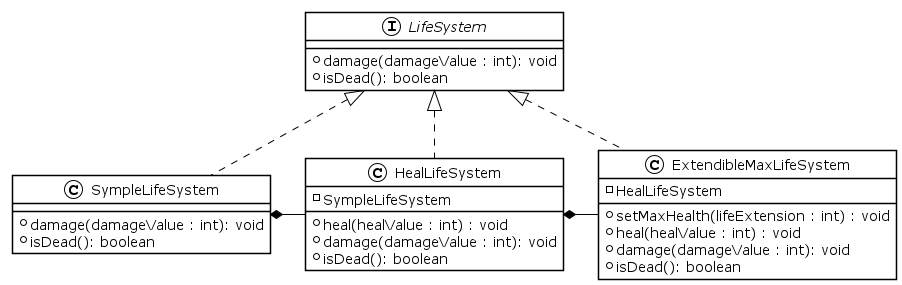
\includegraphics[scale=0.45]{img/uml/LifeSystem.png}
    \caption{Life system}
    \label{fig: Life system}
\end{figure}
\par \noindent Durante la progettazione si è deciso che ogni personaggio (giocatore e nemici) potesse avere un sistema di vita differente. Questi però presentano sia similarità che differenze. Per esempio sia il nemico che il giocatore possono ricevere danno e morire mentre solo quest’ultimo può curarsi ed estendere la propria vita. 
Per rispettare queste premesse ho implementato un sistema “a cascata”. 
\par \noindent L’idea é quella che un sistema più complesso si occuperà solamente di gestire le funzionalità avanzate e utilizzi un sistema più semplice per svolgere le operazioni in comune. 
\par \noindent Utilizzare classi semplici per creare sistemi più complessi mi ha permesso di ridurre la ripetizione di codice e aumentarne il riuso. 


\newpage
\paragraph{Artefatti}
\par \noindent \\
\begin{figure}[H]
    \centering
    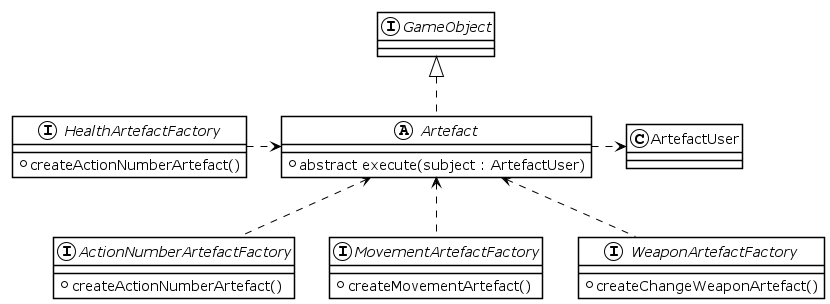
\includegraphics[scale=0.55]{img/uml/Artefact.png}
    \caption{Artefatti}
    \label{fig: Artefatti}
\end{figure}
\par \noindent Gli artefatti sono modificatori di statistiche che permettono al giocatore di cambiare arma, curarsi, estendere la propria vita e aumentare il numero di azioni per turno. 
Per l’implementazione ho deciso di creare una classe astratta, definendo al suo interno la parte comune a tutti gli artefatti,  lasciando un metodo astratto execute.
\par \noindent Questo metodo andrà a direttamente a chiamare i metodi corrispondenti all’effetto sull’utilizzatore e sarà quindi diverso per ogni artefatto. 
\par \noindent Per la creazione degli artefatti ho deciso di utilizzare il \textit{pattern Factory}. Questo pattern ha due vantaggi principali. Il primo è quello di offrire all’utilizzatore una interfaccia semplice per la loro creazione mentre il secondo riguarda i futuri sviluppi in quanto sarà possibile introdurre nuovi artefatti in gioco senza dover modificare ulteriori classi se non la Factory già esistente. 
\par \noindent Ogni tipologia di artefatti possiede una Factory differente per la propria creazione.

\newpage
\paragraph{Moving Strategy}
\par \noindent \\
\begin{figure}[H]
    \centering
    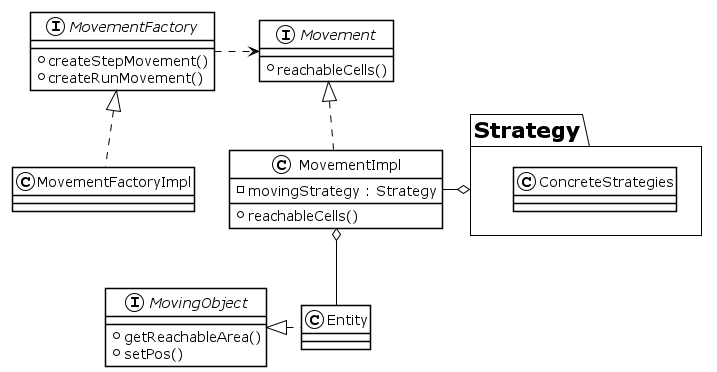
\includegraphics[scale=0.6]{img/uml/Movement.png}
    \caption{Strategie di movimento}
    \label{fig: Strategie di movimento}
\end{figure}
\par \noindent Questa parte del progetto è atta a incapsulare il sistema di movimento delle entità mobili all’interno della griglia di gioco. Lo scopo è quello di fornire al controller le possibili posizioni che potrà assumere un oggetto in grado di spostarsi durante il proprio turno.
\par \noindent Il sistema di movimento però può cambiare a seconda di chi lo implementa, ad esempio gli zombie si muoveranno in maniera differente dal personaggio principale, e il personaggio principale deve essere in grado di poter cambiare moving strategy tramite l’utilizzo degli artefatti. 
\par \noindent Per questo motivo si è deciso di utilizzare il \textit{pattern Strategy}. Questo pattern infatti permette di rendere indipendente l’utilizzatore del sistema di movimento dall'algoritmo che questo incapsula. 
\par \noindent Il pattern si compone dell’interfaccia Strategy, che viene poi implementata in diverse classi, ognuna con caratteristiche diverse. Il contesto del pattern strategy è rappresentato dalla classe MovementImpl, mentre l’utilizzatore é una classe che estende MovingObject, in questo caso Entity. 
\par \noindent Per cambiare sistema di movimento sará poi possibile  andare a sostituire l’intera classe MoventImpl all’interno dell’utilizzatore.
\par \noindent Per la creazione delle classi MovementImpl è stato utilizzato il \textit{pattern Factory}. Questa scelta é stata fatta con l’ottica di facilitarne la creazione e l’espandibilità futura.

\subsubsection*{\large \slshape Federico Bartolini}
\paragraph{Schermata di Vittoria e Sconfitta}
\par \noindent \\
\begin{figure}[H]
    \centering
    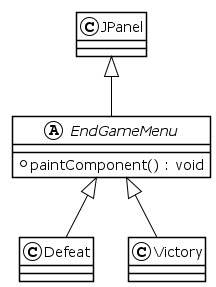
\includegraphics[scale=0.8]{img/uml/EndGameMenu.png}
    \caption{Schermata di Vittoria e Sconfitta}
    \label{fig: Schermata di Vittoria e Sconfitta}
\end{figure}
\par \noindent In questa classe astratta, l’applicazione mostra al giocatore una schermata, dedicata all’avverarsi delle condizioni di vittoria e sconfitta. Ho utilizzato una classe astratta per evitare ripetizione di codice, in modo tale da renderlo più leggibile e meno complicato.

\paragraph{Ostacoli}
\par \noindent \\
\begin{figure}[H]
    \centering
    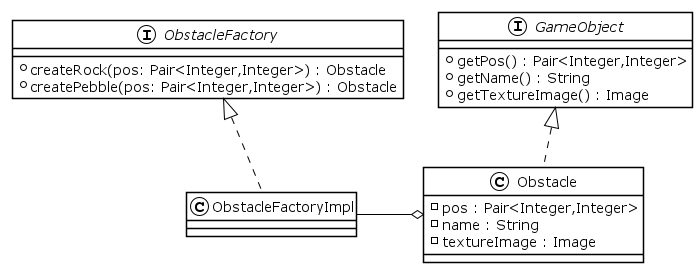
\includegraphics[scale=0.55]{img/uml/Obstacle.png}
    \caption{Ostacoli}
    \label{fig: Ostacoli}
\end{figure}
\par \noindent Esistono per ora due tipi di ostacoli creati all’interno della classe Obstacle
Per ora, i soli due ostacoli sono sassi e sassolini che hanno la stessa funzione, ovvero “bloccare” la strada sia ai nemici che al personaggio. Nonostante tutto, sarà possibile attaccare attraverso essi.
\par \noindent Nel futuro, abbiamo intenzione di aggiungerne altri con azioni di non solo blocco, ma che possano fare in modo di essere utilizzati come elementi che ti fanno perdere vita, o trappole per cui il giocatore perda la partita.

\paragraph{Menù d'azione}
\par \noindent \\
\begin{figure}[H]
    \centering
    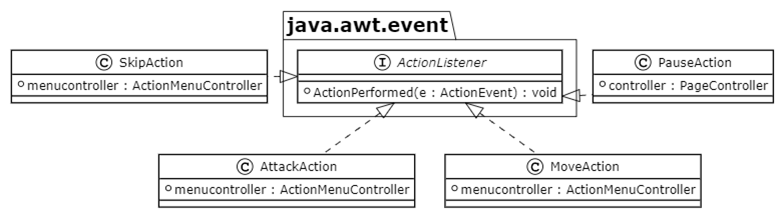
\includegraphics[scale=0.5]{img/uml/ActionMenu.png}
    \caption{Menù d'azione}
    \label{fig: Menù d'azione}
\end{figure}
\par \noindent Il menù di azione sarà contenuto all’interno del TotalPanel, e sarà composto da quattro pulsanti, che ci permettono di attaccare, muovere, saltare il turno e di mettere il gioco in pausa.
\par \noindent Ogni pulsante viene gestito tramite un ActionListener che, a seconda del bottone premuto, ci permette di eseguire la determinata azione. Le azioni di attacco, movimento e turno saltato sono controllate dal GameController, come vedremo tra poco, mentre nel caso in cui il gioco venga interrotto viene controllato dal PageController.
\newpage
\paragraph{Gestione del turno del Player (Attacco e Movimento)}
\par \noindent \\
\begin{figure}[H]
    \centering
    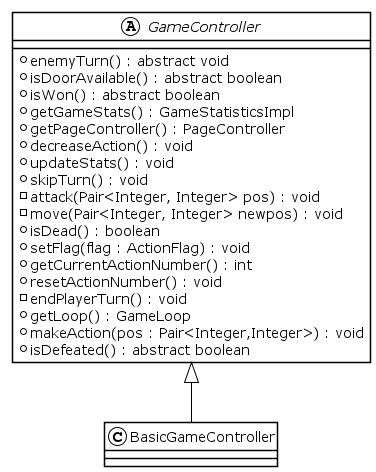
\includegraphics[scale=0.7]{img/uml/GameController.png}
    \caption{Turno del Player}
    \label{fig: Turno del Player}
\end{figure}
\par \noindent All’interno del turno, il player ha a disposizione un numero limitato di azioni, che viene inizializzato a 2. Le azioni che il giocatore può effettuare all’interno del turno stesso sono : la possibilità di attaccare, la possibilità di muoversi e, volendo se lo ritiene necessario, la possibilità di saltare il turno corrente (non vengono diminuite il numero d’azioni correnti, ma vengono direttamente portate a 0, facendo di conseguenza iniziare un nuovo turno al player con il conseguente movimento o attacco da parte dei nemici).
\par \noindent Il tutto viene gestito all’interno del GameController il quale si occupa di attaccare, muovere o saltare il turno.
\newpage
\paragraph{Menù di Pausa}
\par \noindent \\
\begin{figure}[H]
    \centering
    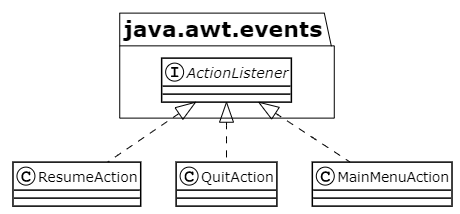
\includegraphics[scale=0.7]{img/uml/PauseMenu.png}
    \caption{Menù di Pausa}
    \label{fig: Menù di Pausa}
\end{figure}
\par \noindent Il menù di pausa è una schermata contenente tre pulsanti di cui ognuno può eseguire una determinata azione.
\par \noindent Tutte le azioni dei pulsanti vengono effettuate tramite la classe Controller.
\newpage

\subsubsection*{\large \slshape Samuele De Tuglie}
\paragraph{Struttura della stanza}
\par \noindent \\
\begin{figure}[H]
    \centering
    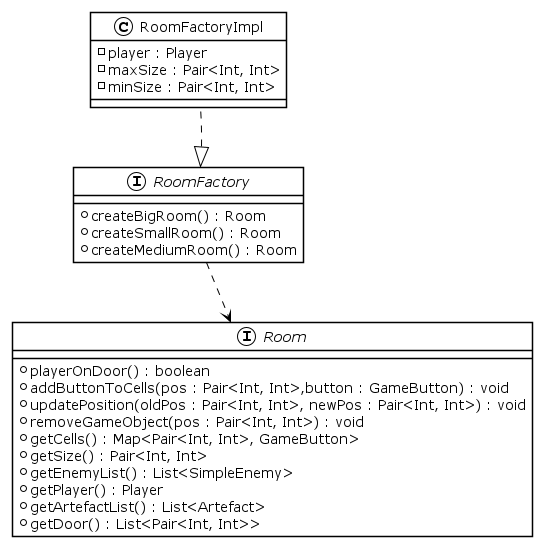
\includegraphics[scale=0.7]{img/uml/Room.png}
    \caption{Generazione della stanza}
    \label{fig: Stanza}
\end{figure}
\par \noindent Esistono tre tipi di stanze, una piccola, una media e una grande, generati utilizzando il  \textit{pattern Factory}. La dimensione della stanza piccola e della stanza grande è data dalla dimensione del monitor, mentre la dimensione della stanza media è data dalla media delle dimensioni della stanza piccola e grande così da poter giocare con ogni tipo di monitor senza problemi.
\begin{figure}[H]
    \centering
    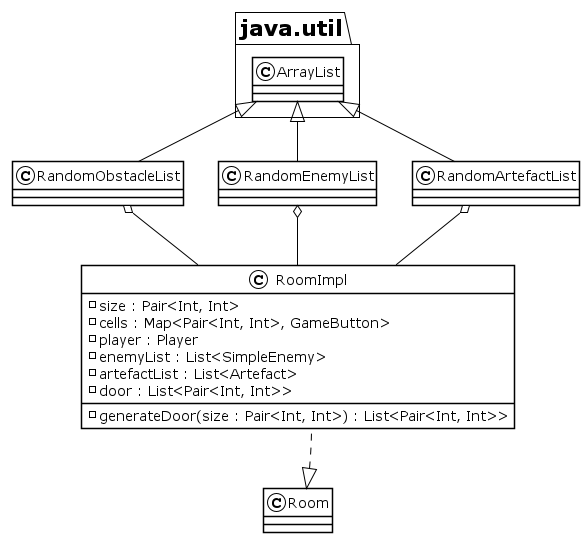
\includegraphics[scale=0.7]{img/uml/Room2.png}
    \caption{Generazione Game Object nella stanza}
    \label{fig: Stanza}
\end{figure}
\par \noindent Il numero di nemici e di artefatti è uguale, ed è calcolato in base alla grandezza della stanza. Ogni tipo di stanza ha un punto predefinito di spawn del player. La porta per cambiare stanza viene generata nell’ultima colonna a destra.
\newpage
\paragraph{Schermata di caricamento}
\par \noindent \\
\begin{figure}[H]
    \centering
    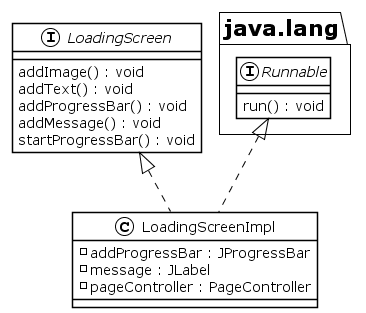
\includegraphics[scale=0.7]{img/uml/loading_screen.png}
    \caption{Schermata di caricamento}
    \label{fig: Loading screen}
\end{figure}
\par \noindent Al fine di alleggerire graficamente il programma, ho voluto implementare una schermata di caricamento, che viene mostrata durante la creazione dell’area di gioco che è la parte più pesante del programma.
\newpage
\paragraph{Area di gioco}
\par \noindent \\
\begin{figure}[H]
    \centering
    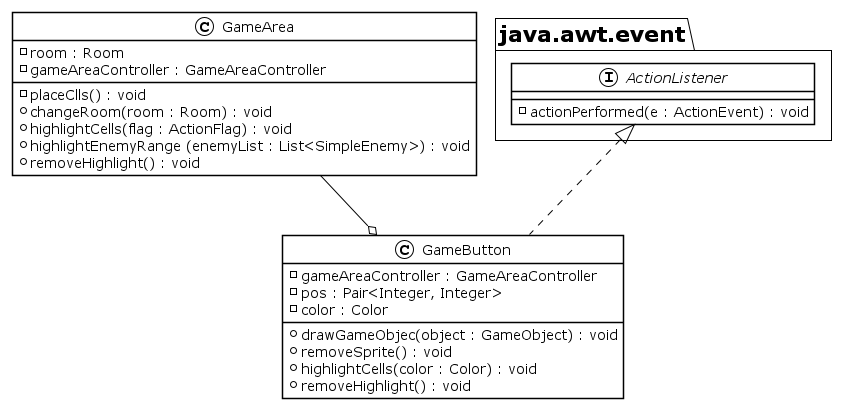
\includegraphics[scale=0.55]{img/uml/GameArea.png}
    \caption{Area di gioco nella view}
    \label{fig: Game Area nella view}
\end{figure}
\par \noindent L’area di gioco è la zona che rappresenta graficamente la stanza (e tutti gli oggetti da essa contenuti, come i nemici, gli artefatti o gli ostacoli).
Quando l’utente sceglie di fare un’azione, premendo per esempio il bottone “Move”, allora tutte le celle in cui il Player si può muovere si illumineranno e si sbloccheranno, permettendogli di compiere l’azione desiderata.
\begin{figure}[H]
    \centering
    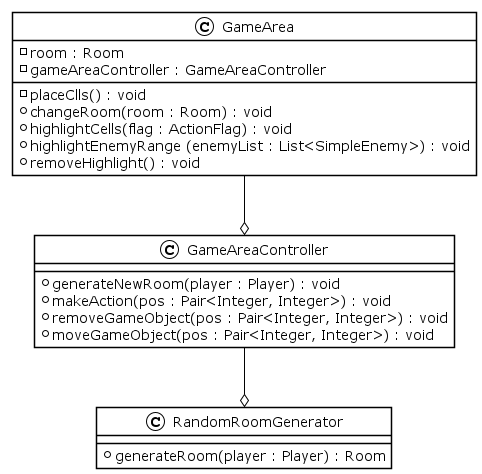
\includegraphics[scale=0.7]{img/uml/GameArea2.png}
    \caption{Area di gioco nel controller}
    \label{fig: Game Area nel controller}
\end{figure}
\par \noindent Alla pressione dei bottoni viene chiamata la classe GameAreaController, una classe creata con lo scopo di separare la view dal controller, per seguire al meglio il pattern MVC.
Quando il Player sale sopra la porta viene caricata e mostrata un'altra stanza.

\paragraph{Gui scalabile}
\par \noindent \\
Al fine di rendere ottimale l’esperienza di gioco, ho optato per creare dei metodi e degli oggetti che si adattino in base al monitor, per esempio la dimensione della stanza, oppure tutte le immagini inserite (scalano usando la classe ImageModifier, permettendo sia di mantenere il rapporto dell’immagine, sia di allungarla).

\subsubsection*{\large \slshape Sara Romeo}

\paragraph{Turno nemico}
\par \noindent \\
\begin{figure}[H]
    \centering
    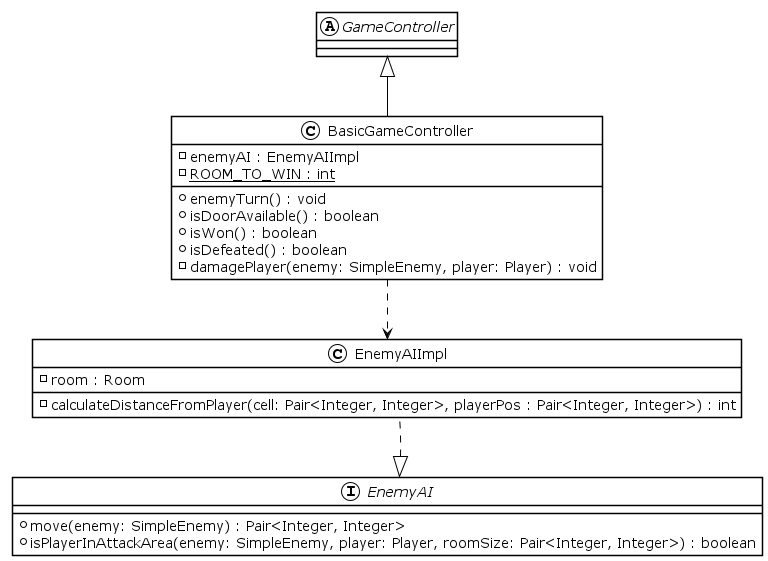
\includegraphics[scale=0.5]{img/uml/EnemyAI.png}
    \caption{AI nemica}
    \label{fig: AI nemica}
\end{figure}
\par \noindent L'idea dietro al Basic Game Controller è quella di mantenere aperta la possibilità di definire diverse modalità di gioco in un futuro ampliamento dell'applicativo.
\par \noindent Con quest'obbiettivo in mente, il \textit{Template Method Pattern} si è rivelato particolarmente conveniente. In questo caso l'unica condizione di vittoria è il superamento di 3 stanze, indipendentemente dall'eliminazione di nemici.
Grazie alla struttura stabilita è stato possibile specializzare alcuni aspetti della tipologia di gioco quali:
\begin{itemize}
    \item[--] \textit{Condizioni di vittoria o sconfitta}
    \item[--] \textit{Disponibilità della porta}, per passare alla stanza successiva quando il giocatore vi si muove sopra
    \item[--] \textit{Turno nemico}, in particolare:\\
		gli zombie attaccano tutti prima che il player possa compiere altre azioni al turno successivo. Se il giocatore è nell'area nemica di attacco, verrà colpito, nel caso contrario lo zombie si avvicinerà al protagonista.
\end{itemize}
\par \noindent Per stabilire come lo zombie si sposti si è scelto di esternalizzare un'AI nemica per decidere in base alla movement strategy che possiede e dove si trova il player: la casella scelta sarà quella che permette di approcciarsi di più a Marcello. Scorporando la scelta algoritmica del turno (se lo zombie deve attaccare o muoversi) da quella automatizzata di quale sia la miglior posizione in cui spostarsi sarà più semplice cambiare il processo automatizzato di scelta nemica.

\paragraph{Diverse armi e nemici}
\par \noindent \\
\begin{figure}[H]
    \centering
    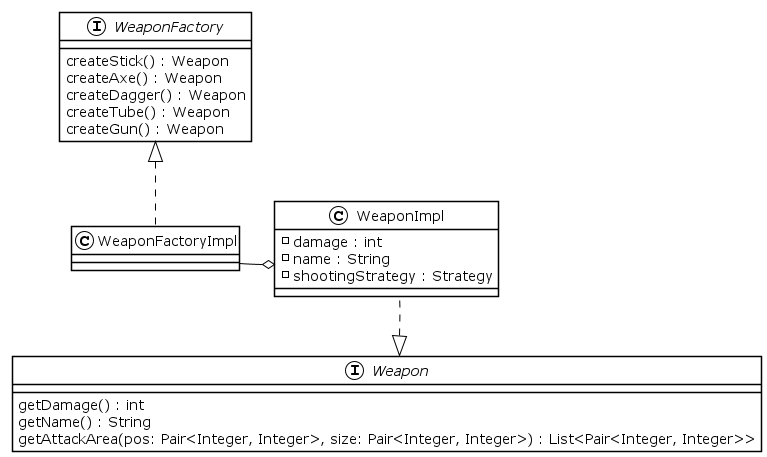
\includegraphics[scale=0.55]{img/uml/Weapon.png}
    \caption{Armi diverse.}
    \label{fig: Weapon}
\end{figure}
\begin{figure}[H]
    \centering
    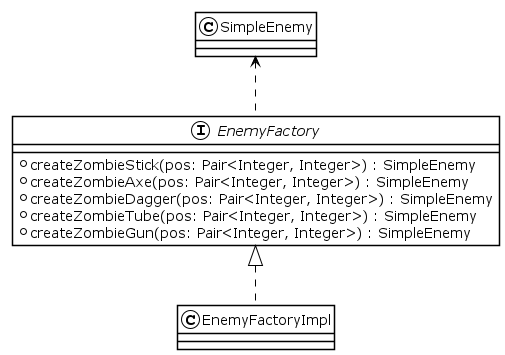
\includegraphics[scale=0.7]{img/uml/Enemy.png}
    \caption{Nemici diversi.}
    \label{fig: Enemy}
\end{figure}
\par \noindent Per riuscire ad implementare diverse tipologie di armi e nemici, combinando diverse caratteristiche, si è optato per il \textit{Factory Pattern}. Ogni arma così avrà strategie di attacco e ammontare dei danni differenti, mentre sarà possibile mantenerne comune lo scheletro delle funzionalità.
\par \noindent Grazie a questa scelta, in futuro sarà più semplice decidere di aumentare le tipologie e implementare nuove peculiarità delle armi.
\par \noindent Per le stesse motivazioni anche la creazione dei nemici è stata serializzata col \textit{Factory Pattern}. Qui è dove, per assegnare un'arma a un tipo di zombie, ci si è avvalsi dell'utilizzo della factory di armi.
\par \noindent Per quanto riguarda il range di attacco, come già anticipato in precedenza, si è optato per il \textit{Strategy Pattern}, che ha permesso di condividere le stesse implementazioni delle strategie di movimento. È stata inoltre aggiunta una concrete strategy e modificatori di distanza per ognuna, così da permettere maggiore varietà di range di attacco delle armi.
\newpage
\paragraph{Statistiche di gioco e log}
\par \noindent \\
\begin{figure}[H]
    \centering
    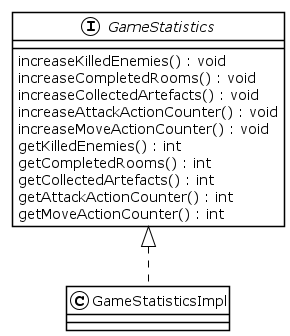
\includegraphics[scale=0.8]{img/uml/GameStatistics.png}
    \caption{Statistiche di gioco}
    \label{fig: Game Statistics}
\end{figure}
\par \noindent Per riuscire a tenere conto dei dati della partita si è optato per la creazione di un'utility Counter, di cui è stato possibile sfruttare le funzionalità all'interno delle Game Statistics. Le statistiche di gioco prese in esame sono il numero di stanze completate, il totale di nemici uccisi, il numero di artefatti raccolti e il numero di azioni di tipo attacco o movimento.
Queste sono importanti a livello di model in quanto, sempre in vista di diverse modalità di gioco, lasciano ad esempio la possibilità di definire più facilmente molteplici condizioni di vittoria differenti diverse.
\par \noindent Allo stesso tempo le stesse hanno anche un utilizzo informativo per l'utente, in quanto vengono mostrate insieme ai dati del player e al numero di azioni rimaste, all'interno delle Stats.
\begin{figure}[H]
    \centering
    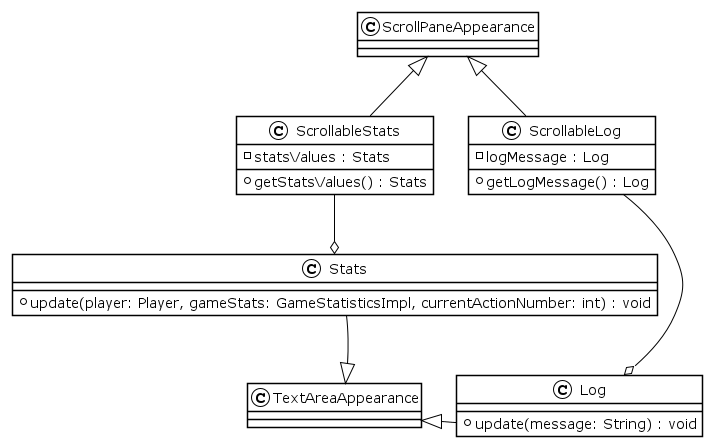
\includegraphics[scale=0.55]{img/uml/StatsLog.png}
    \caption{Statistiche e Log}
    \label{fig:Statistiche e log}
\end{figure}
\par \noindent Le aree laterali della schermata di gioco sono rispettivamente sulla sinistra le statistiche e a destra i log della partita, parte di View.
\par \noindent I log vengono implementati all'interno degli algoritmi di gioco nel controller: a seconda di ciò che è appena successo e/o serve all'utente tenere traccia all'interno della partita viene inviata una stringa che spiega la situazione.
\par \noindent Si è scelto di scorporare l'aspetto estetico dalla funzionalità delle rispettive aree, impostando classi contenenti l'aspetto.

\newpage
\section{Sviluppo}
\subsection{Testing automatizzato}
Durante lo sviluppo del progetto abbiamo scelto di effettuare dei test per alcuni algoritmi specifici per assicurarne il funzionamento una volta giunti al termine. Segue un elenco dei componenti verificati con relativa spiegazione a riguardo.
\begin{itemize}
    \item Strategy:
        \begin{itemize}
            \item[\ding{51}] AroundAreaTest
            \item[\ding{51}] AsteriskAreaTest
            \item[\ding{51}] CrossAreaTest
        \end{itemize}
    \par \noindent Si è verificato che l'area desiderata corrispondesse alle celle considerate dai rispettivi algoritmi delle strategy.
    \item Life system:
        \begin{itemize}
            \item[\ding{51}] ExtendibleMaxLifeSystemTest
            \item[\ding{51}] HealLifeSystemTest
            \item[\ding{51}] SimpleLifeSystemTest
        \end{itemize}
    \par \noindent Controllo del corretto funzionamento dei diversi life system, accertandosi che il danno ricevuto dall'entità fosse effettivamente assorbito.
    \item Enemy AI (movimento):
        \begin{itemize}
            \item[\ding{51}] EnemyAITest
        \end{itemize}
    \par \noindent Verifica che per ogni strategia di movimento nemica lo zombie, ovunque il player si trovi, si avvicini nella maniera corretta.
    \item Entity:
        \begin{itemize}
            \item[\ding{51}] PlayerTest
            \item[\ding{51}] SimpleEntityTest
        \end{itemize}
    \par \noindent Si accerta che le classi che modellano le entità funzionino correttamente. Per entrambi viene testata la creazione e il sistema di vita, mentre solo per la classe Player viene testato l’effettivo funzionamento degli artefatti.
    \newline
    \item Stanza ed elementi che vi interagiscono
        \begin{itemize}
            \item[\ding{51}] {PosInGridTest}
            \newline Controlla che la posizione sia all'interno della griglia di gioco.
            \item[\ding{51}] {RoomTest}
            \newline Controlla la creazione della stanza.
            \item[\ding{51}] GameObjectSpawnTest
            \newline Per verificare che gli oggetti creati usando le reflection siano giusti.
        \end{itemize}
\end{itemize}

\subsection{Metodologia di lavoro}
Si è cercato di mantenere lo sviluppo del progetto il più scorporato e indipendente possibile tra i componenti. Questa è stata anche una scelta al fine di poter lavorare in parallelo evitando problemi quali merge conflit, creando branch per ogni funzione e relativi hotfix e refactor. Si è stabilito che il branch dev fosse la base di sviluppo, mentre il main è rimasto invariato fino alla prima release. Chiaramente alcuni step hanno richiesto un confronto più approfondito per prendere importanti decisioni strutturali, in particolare la prima fase di analisi e progettazione generica dell'applicativo per permettere di accordarsi sugli scopi e il lavoro da svolgere. Per una programmazione più efficiente qui sono state definite generiche interfacce per rendere il piano complessivo del gioco da creare. Queste poi sono state divise e prese in analisi singolarmente da ognuno e di conseguenza hanno subito modifiche a seconda delle necessità e delle scelte di pattern e composizione pratica del codice.
\par \noindent Come già denotato in fase di analisi e integrando successivamente:
\begin{itemize}
    \item[\ding{228}] {\slshape Luca Babboni:} sistema di cura e gestione degli oggetti, creazione personaggio e bilanciamento statistiche, menù principale, strategie di movimento.
    \item[\ding{228}] {\slshape Federico Bartolini:} gestione del turno del player (movimento, attacco), interfaccia del menù d'azione, menù di pausa, ostacoli, schermate di vittoria e sconfitta.
    \item[\ding{228}] {\slshape Samuele De Tuglie:} interfaccia grafica, collegamento e creazione di stanze (modello della stanza, spawn di game object), schermata di caricamento.
    \item[\ding{228}] {\slshape Sara Romeo:} generazione di nemici e armi differenti, visualizzazione log e statistiche, turno dei nemici con relativa AI, condizioni di vittoria.
\end{itemize}

\subsection{Note di sviluppo}
\subsubsection*{\large \slshape Luca Babboni}
\begin{itemize}
    \item[\ding{223}] Lambda Expressions
    \item[\ding{223}] Optional
\end{itemize}

\subsubsection*{\large \slshape Federico Bartolini}
\begin{itemize}
    \item[\ding{223}] Lambda Expressions
\end{itemize}

\subsubsection*{\large \slshape Samuele De Tuglie}
\begin{itemize}
    \item[\ding{223}] Reflection
\end{itemize}

\subsubsection*{\large \slshape Sara Romeo}
\begin{itemize}
    \item[\ding{223}] Stream
    \item[\ding{223}] Lambda Expressions
\end{itemize}
Si è ritenuta utile l'implementazione di una classe che modelli un sistema di coordinate e l'inserimento di un sistema di conteggio. Per questo si è scelto rispettivamente di riusare il codice relativo ai Pair e riadattare il Counter, visti durante il corso.

\newpage
\section{Commenti finali}
\subsection{Autovalutazione e lavori futuri}
\subsubsection*{\large \slshape Luca Babboni}
\par \noindent Questo progetto mi ha permesso di approcciarmi per la prima volta all’esperienza dello sviluppo software in gruppo, che sono sicuro mi tornerá molto utile in futuro, e di prendere familiarità all'utilizzo di Git e GitHub. 
\par \noindent Al momento il gioco si presenta come un concept per un possibile sviluppo futuro che potrebbe essere migliorato cambiando alcune dinamiche, al fine di creare un gameplay piú complesso. 
\par \noindent Mi ritengo soddisfatto del codice che ho realizzato, nel quale ho cercato di seguire i principi di programmazione a oggetti che ho seguito  a lezione. 


\subsubsection*{\large \slshape Federico Bartolini}
\par \noindent Inizialmente, non ero effettivamente convinto di questo progetto data la sua “complessità”, ma considerando il prodotto finale sono veramente soddisfatto. Sono sicuro che tutte le cose che imparate in questo periodo mi torneranno utili in un futuro.
\par \noindent Inoltre, mi ritengo altrettanto soddisfatto per quanto riguarda il fare gruppo, in quanto normalmente sono abituato a lavorare in singolo, e questa esperienza più di gruppo mi ha decisamente aiutato.

\subsubsection*{\large \slshape Samuele De Tuglie}
\par \noindent L’ho ritenuto un progetto all’inizio difficile, per vie di complicazioni come l’utilizzo di git a cui personalmente non ero ancora molto abituato, inoltre in passato ho avuto poche occasioni di lavorare in gruppo, quindi ho ritenuto complicato anche fare cose basilari come coordinarsi con gli altri o comunque mettersi d’accordo con tutti. 
\par \noindent Anche se ho avuto esperienze passate con java già alle superiori, non mi sono mai sentito troppo bravo in argomento, quindi comunque ho colto l’occasione per migliorare. 
In conclusione le mie preoccupazioni si sono dissolte e ho ritenuto il tutto molto formativo.

\subsubsection*{\large \slshape Sara Romeo}
\par \noindent All'inizio ero in pensiero sia per il quantitativo di capacità e tecniche di programmazione a me nuove richieste sia per il dover organizzare un lavoro di queste dimensioni all'interno del gruppo.
\par \noindent Ora sono molto contenta di aver avuto quest'occasione per poter arricchire le mie conoscenze e vederle applicate, inoltre mi sento soddisfatta e grata di aver avuto al mio fianco compagni di lavoro collaborativi. È stato molto impegnativo, ma altrettanto istruttivo e utile, un'ottima occasione per crescere.

\newpage
\appendix
\section{Guida Utente}

\subsection*{Controlli}
Ad ogni turno le azioni possono effettuare tramite semplice utilizzo del mouse. Si sceglie l'azione dal menu in basso, se attacca o muove si clicca sulla casella colorata dove si vuole compiere l'azione.

\subsection*{Artefatti}
\begin{itemize}
    \begin{figure}[H]
    	\item[\textbf{ }]
    	
\includegraphics[width=0.05\linewidth]{img/rsc/Big_Heal}
		\label{img:Big_Heal}
		\textbf{BIG HEAL}\\
  		\underline{CURA}: Cura molto Marcello.
	\end{figure}
	    
	\begin{figure}[H]
		\item[\textbf{ }]
		
\includegraphics[width=0.05\linewidth]{img/rsc/Little_Heal}
		\label{img:Little_Heal}
		\textbf{LITTLE HEAL}\\
        \underline{CURA}: Cura poco Marcello.
	\end{figure}
	    
    \begin{figure}[H]
		\item[\textbf{ }]
		
\includegraphics[width=0.05\linewidth]{img/rsc/Health_Extender}
		\label{img:Health_Extender}
		\textbf{HEALTH EXTENDER}\\
        \underline{CURA}: Estende la vita di Marcello.
    \end{figure}

    \begin{figure}[H]
		\item[\textbf{ }]
		
\includegraphics[width=0.05\linewidth]{img/rsc/Action_Number_Increaser}
		\label{img:Action_Number_Increaser}
		\textbf{ACTION NUMBER INCREASER}\\
		\underline{AZIONI}: Aumenta il numero di azioni per turno.
	\end{figure}
    
	\begin{figure}[H]
		\item[\textbf{ }]
		
\includegraphics[width=0.05\linewidth]{img/rsc/Run}
		\label{img:Run}
		\textbf{RUN}\\
        \underline{MOVIMENTO}: Permette di muoversi di due caselle in verticale o in orizzontale rispetto a Marcello.
    \end{figure}
    	
	\begin{figure}[H]
		\item[\textbf{ }]
		
\includegraphics[width=0.05\linewidth]{img/rsc/Step}
		\label{img:Step}
		\textbf{STEP}\\
        \underline{MOVIMENTO}: Permette di muoversi di una casella tra quelle intorno a Marcello.
    \end{figure}
    
    \begin{figure}[H]
		\item[\textbf{ }]
		
\includegraphics[width=0.05\linewidth]{img/rsc/Axe}
		\label{img:Axe}
		\textbf{AXE}\\
        \underline{ARMA}: Ascia, taglia nelle celle intorno
    \end{figure}
    
    \begin{figure}[H]
		\item[\textbf{ }]
		
\includegraphics[width=0.05\linewidth]{img/rsc/Dagger}
		\label{img:Dagger}
		\textbf{DAGGER}\\
        \underline{ARMA}: Pugnale, trafigge nelle celle circostanti
    \end{figure}
    
    \begin{figure}[H]
		\item[\textbf{ }]
		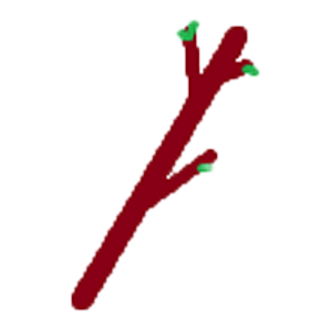
\includegraphics[width=0.05\linewidth]{img/rsc/Stick}
		\label{img:Stick}
		\textbf{STICK}\\
        \underline{ARMA}: Bastone, colpisce nelle celle intorno
    \end{figure}
    
    \begin{figure}[H]
		\item[\textbf{ }]
		
\includegraphics[width=0.05\linewidth]{img/rsc/Tube}
		\label{img:Tube}
		\textbf{TUBE}\\
        \underline{ARMA}: Tubo, colpisce nelle caselle circostanti, ma non nella casella a destra e a sinistra
    \end{figure}
    
    \begin{figure}[H]
		\item[\textbf{ }]
		
\includegraphics[width=0.05\linewidth]{img/rsc/Gun}
		\label{img:Gun}
		\textbf{GUN}\\
        \underline{ARMA}: Pistola, proiettili con raggio due caselle
    \end{figure}
\end{itemize}

\subsection*{Ostacoli}
\begin{itemize}
    \begin{figure}[H]
		\item[\textbf{ }]
		
\includegraphics[width=0.05\linewidth]{img/rsc/Pebble.png}
		\label{img: Pebble}
		\textbf{Ciottoli}\\
        \underline{BLOCCO}: Marcello non calpesta i sassolini.
    \end{figure}
    
    \begin{figure}[H]
		\item[\textbf{ }]
		
\includegraphics[width=0.05\linewidth]{img/rsc/Rock.png}
		\label{img: Rock}
		\textbf{Roccia}\\
        \underline{BLOCCO}: Marcello non può stare sopra una roccia.
    \end{figure}
\end{itemize}

\subsection*{Celle colorate}
\begin{itemize}
    \begin{figure}[H]
		\item[\textbf{ }]
		
\includegraphics[width=0.05\linewidth]{img/red}
		\label{img:Stick}
		\textbf{Celle rosse}\\
        \underline{AZIONE}: Dove Marcello può attaccare.
    \end{figure}
    
    \begin{figure}[H]
		\item[\textbf{ }]
		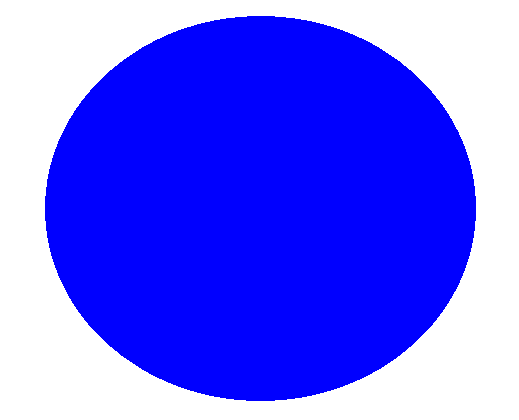
\includegraphics[width=0.05\linewidth]{img/blu}
		\label{img:Tube}
		\textbf{Celle blu}\\
        \underline{AZIONE}: Dove Marcello può spostarsi.
    \end{figure}
    
    \begin{figure}[H]
		\item[\textbf{ }]
		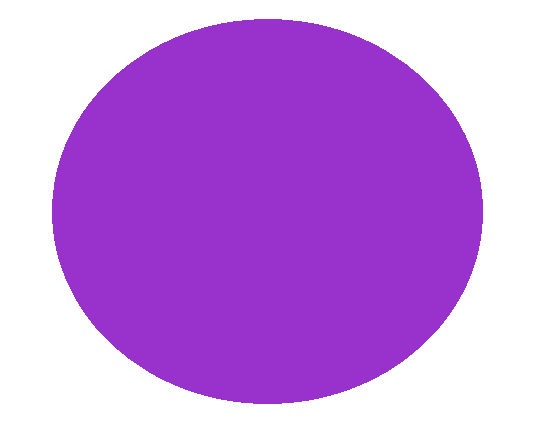
\includegraphics[width=0.05\linewidth]{img/purple}
		\label{img:Gun}
		\textbf{Celle viola}\\
        \underline{CELLA}: Dove i nemici possono attaccare.
    \end{figure}
\end{itemize}

\end{document}